\documentclass[a4paper,twocolumn]{article}
%  
\usepackage{amssymb}
\usepackage{amsmath}
\usepackage{physics}
% \usepackage{siunitx}
\usepackage{graphicx}
\graphicspath{{./graph/}}

%*****RELAZIONE DOMINIO FREQUENZA*****

\begin{document}

\title{Use of Operational Amplifier as  an Integrator and Differentiator}
\author{{Stefano Pilosio}}

\maketitle

\section{Abstract}
Our group measured the frequency response of two similar circuits, that , while using the same components, show opposing behavior, not only in the resulting waveform, but also in the frequency Response.

\section{Introduction}

\subsection{Operational Amplifier} 

The circuits are composed of a resistor ($R$), a capacitor ($C$) and an operational amplifier. To analyze their behavior we need to know the functioning of an ideal operational amplifier, herein known as ``OPAMP''.

The ideal OPAMP is a voltage-controlled voltage source, with a voltage gain $E = \frac{V_o}{V_i}$, where $V_o$ is the output voltage and $V_i$ is the input voltage, in this case $V_o$ is referenced to ground, while $V_i$ is the voltage difference between two poles, that are known as inverting ($V^+$) and not inverting ($V^-$) inputs, so $V_i=V^+-V^-$. In the ideal OPAMP $E\to\infty$.

To run the circuit in the desired configuration we have to use a negative feedback loop, in this way we can use \emph{virtual short circuit principle}, this is related to the stability of negative feedback and $E\to\infty$, due to this factor $V^+-V^-=0$, it is also named 'Virtual Ground' because often the not-inverting input is at ground potential, so $V^+=0=V^-$.

\subsection{Integrator Circuit}

% \begin{figure}
%     \centering
%     % \def\svgwidht{\columnwidth}
%     \input{differentiatorCircuit.pdf_tex}
% \end{figure}

As in the figure, in the feedback loop we have a capacitor and a resistor, so writing the Ohm's Law, Capacitor Law ($ q = Cv \implies \dv {q}{t}=i=C\dv{v}{t} $) and KCL we obtain:
\begin{gather*}
    \begin{cases}
        v_{IN} - R\cdot i_R = v^-\\
        i_R=i_C\\
        v^+-v^-=0\\
        v^+=0\\
        i_C=C\dv{v^--v_{OUT}}{t}
    \end{cases}\\
    i = \frac{v_{IN}}{R}=-C\dv{v_{OUT}}{t}\\
\end{gather*}

From last equation, resolving for $v_{OUT}$:
\begin{equation}
\label{eq:Integrator}
    v_{OUT}=-\frac{1}{CR}\int_0^t{v_{IN}}\,dt + v(0)
\end{equation}

It is visible from \eqref{eq:Integrator}, that the behaviour of this circuit in time domain is to produce the integral of the input voltage function.

The frequency response is defined as \[H=\frac{v_{OUT}}{v_{IN}}(f)\]
So to obtain $H$, we apply Fourier Transform (FT) over \eqref{eq:Integrator}:

\begin{gather}
    V_{OUT}=-\frac{1}{CR(j2\pi f)}V_{IN}\\
    H = \frac{V_{OUT}}{V_{IN}} = \frac{1}{RC(j2\pi f)}   
\end{gather}

\begin{center}
    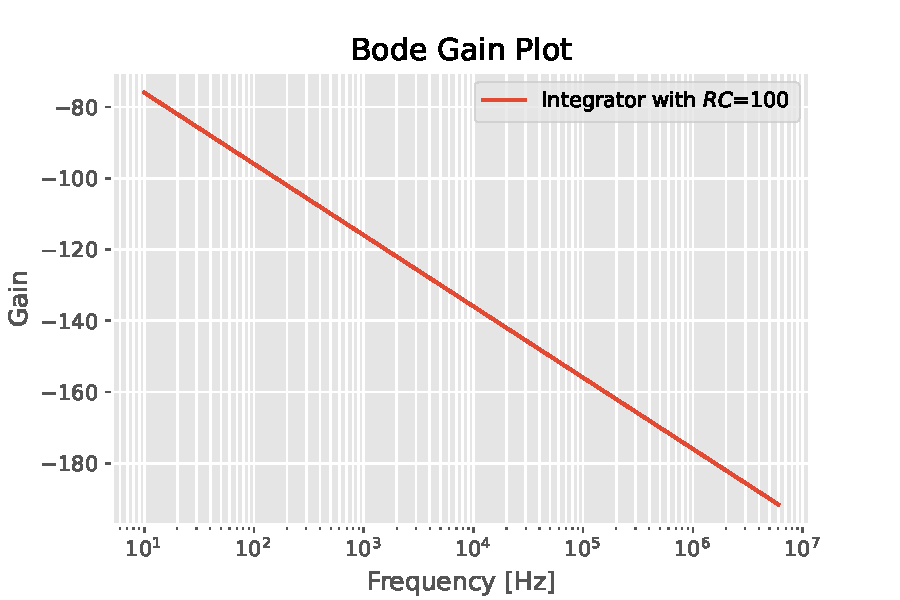
\includegraphics[width=\columnwidth]{graph/IntegratorBodeTheo}
    \label{fig:IntBodeGraphTheo}
\end{center}
Plotting the Bode Gain Diagramm shows a constant negative monotony of -20 dB/dec, this must kept in consideration while using the circuit because it means the output waveform is attenuated with an higher frequency.

\subsection{Differentiator Circuit}

As seen in figure, the circuit is similar to the previous case, but in this case the capacitor and the resistor are swapped. This change produces a completely different response to the input waveform, it can be understood writing KCL, the Ohm's Law and the capacitor law.

\begin{gather*}
    \begin{cases}
        i_C = C\dv{v_{IN}-v^-}{t}\\
        i_R = \frac{v^--v_{OUT}}{R}\\
        i_R = i_C\\
        v^+=v^-\\
        v^-=0
    \end{cases}
    C\dv{v_{IN}}{t}=\frac{-v_{OUT}}{R}
\end{gather*}

As in the precedent case resolving for $v_{OUT}$
\begin{equation}
\label{eq:Differentiator}
    v_{OUT}=RC\dv{v_{IN}}{t}
\end{equation}

\eqref{eq:Differentiator} shows that $v_{OUT}$ is a waveform proportional to the derivative of the input waveform. 

Calculating \(H\) produces:
\begin{gather}
    V_{OUT}=RC\cdot(j2\pi f)V_{IN}\\
    H = RC\cdot(j2\pi f)
\end{gather}

\begin{center}
    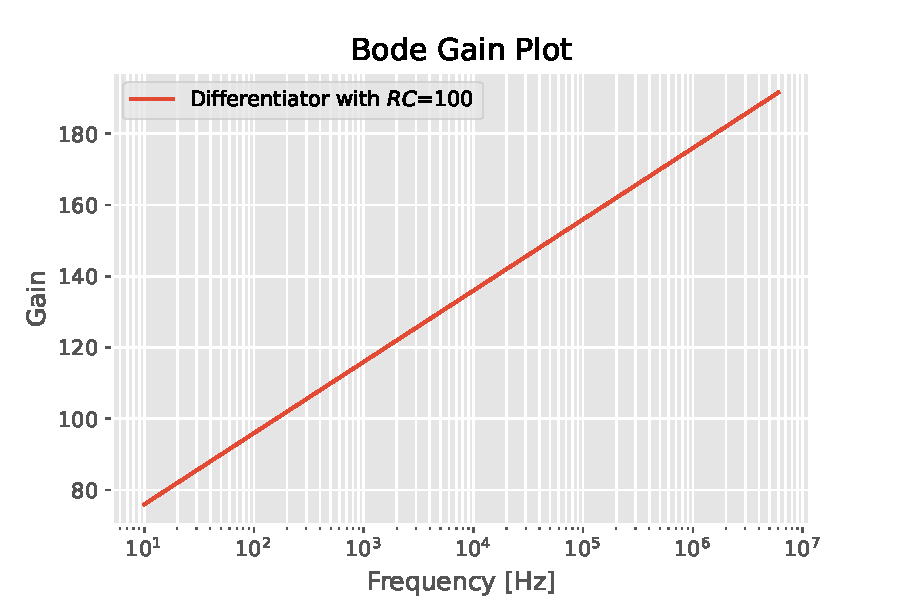
\includegraphics[width=\columnwidth]{graph/DifferentiatorBodeTheo}
    \label{fig:DiffBodeGraphTheo}
\end{center}
In this case the circuit has a constant positive monotony of 20 dB/dec, so with an higher frequency the output signal will be amplified.

\section{Measurement Methods}

% Sottosezone strumenti di misura
\subsection{Materials}
\subsubsection{Instruments}
\begin{itemize}
    \item Oscilloscope ``Tektronix TDS 1012B'';
    \item Function Generator ``Agilent 3322A'';
    \item Power Supply.
\end{itemize}
\subsubsection{Equipment}
\begin{itemize}
    \item OPAMP ``LT081'';
    \item Breadboard;
    \item Wires;
    \item Resistors;
    \item Capacitors;
\end{itemize}
    \subsection{Procedure}

The two circuits are built as shown in the previous pictures, the Oscilloscope probe was connected in the point named \(V_{OUT}\), grounded to ground. The function generator was connected to \(V_{IN}\) and ground. A dual power supply powered the OPAMP, supplying the necessary \(V_{CC+}\) and \(V_{CC-}\). The measure procedure was: set a frequency of the sine wave on the function generator, using the oscilloscope it was measured the voltage peak to peak of the input and the output signal. After that was used the cursor mode on oscilloscope to measure the phase between the two waveforms, for this the cursor was set on time domain and moved in corrispondence of a peak of the input waveform and the nearest peak of the output waveform, at the measure was assigned a positive sign if the output is to the right of input, negative if the output is to the left of input.The frequencies were choosen using an approximate log scale (like 1, 2, 3, 5, 8, 10). 

\section{Analysis}

\subsection{Computation}

During the measuring process datas were saved on a csv file. To analyse  it was used a python enviroment, with the libraries ``\emph{Numpy, Pandas and Matplotlib}'', this enviroment was inserted in a Jupyter Notebook to visualize the results of computation in real time. The code computed and plotted from the data the Bode Diagram and the Nyquist Diagram. At this point it was used another software, ``\emph{NGSpicae}'', to simulate the expected behavior in freqeuncy of the circuits. At this point datas from experiment and simulation are plotted and compared in the python enviroment.

\subsection{Integrator}

\subsection{Differentiator}

\section{Conclusion}

\end{document}